\section{Driver Amplifier}

First, the Driver Amplifier was built. The associated schematic can be
seen in Figure~\ref{DriverAmp}.

\begin{figure}[h!]
  \centering
  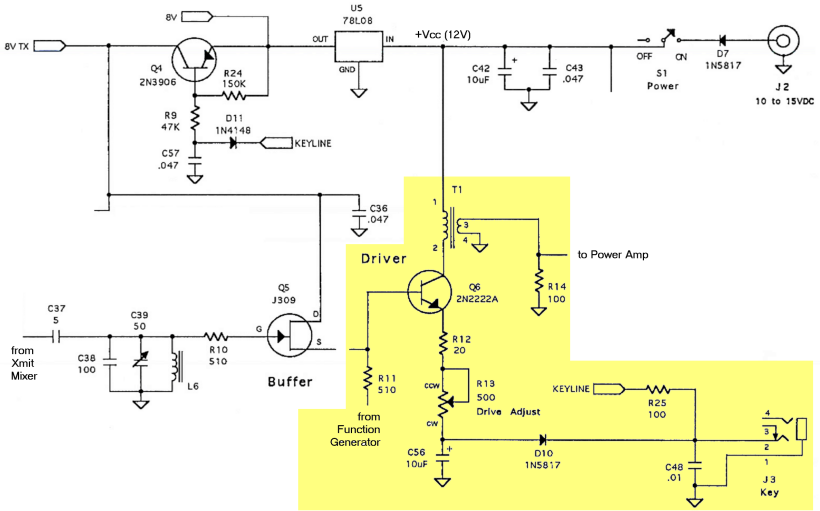
\includegraphics[scale=0.6]{./img/DriverAmp.png}
  \label{DriverAmp}
  \caption{Circuit Schematic for the Driver Amplifier}
\end{figure}

\subsection{Measured Output Voltage: \bm{$V_{out}$}}
With the function generator set to 7.04MHz, and with an offset of 
%Remember to edit this if any changes are made!
$0.5V$. The output voltage across $R_{14}$ was m                      easured
to be $\boxed{2.16 V_{RMS}}$. The voltage observed was high, which threw
off the following calculated values.

\subsection{Calculated Output Power: \bm{$P$}}
  $P$ is calculated using the following:
  \begin{align*}
    P &= \frac{V_{RMS}^2}{R_{14}}
    \implies \frac{2.16^2}{100\Omega}=\boxed{47mW}
  \end{align*}
  %Since $V_{cc}$ is given as $12V$, $R_{14} = 100 \Omega$ and transformer $T_1$ has a turns ratio $n =
  %\frac{14}{4} = 3.5$:
  %\begin{align*}
  %  P &= \frac{12^2}{(3.5^2 \cdot 100}) = \boxed{117.5 mW}
  %\end{align*}
\subsection{Calculated Supply Power: \bm{$P_{0}$}}
\subsubsection{\bm{$V_{R_{12}}$}} 
  The DC voltage across $R_{12}$, $V_{R_{12}}$ was recorded to be
  $\boxed{594 mV}$.
  \subsubsection{\bm{$i_E$}}
  The emitter current, $i_E$, was found by:
  \begin{align*}
    i_E &= \frac{V_{R_{12}}}{R_{12}}
    \implies \frac{595mV}{20\Omega}=\boxed{29.8 mA}
  \end{align*}
  \subsubsection{Supply Power: \bm{$P_0$}}
    $V_{cc}$ was measured at the small resistor across $S_1$, and found to
    be $\boxed{9.72 V}$ Therefore, the DC supply power $P_0 =
    (V_{cc}\cdot i_E)=\boxed{289 mW}$

\subsection{System Efficiency: \bm{$\eta$}}
  The efficiency $\eta$ was calculated to be:
  \begin{align*}
    \eta &= \frac{P}{P_0}
    \implies \frac{47mW}{289mW}\approx\boxed{16\%} 
  \end{align*}

\subsection{Amplifier Gain: \bm{$G$}}
  The gain $G$ was found to be:
  \begin{align*}
    G &= 10log\bigg(\frac{P}{P_0}\bigg) 
    \implies 10log\bigg( \frac{47mW}{289mW}\bigg)=\boxed{-7.9\text{dB}}\\
  \end{align*}
  Since the resistor $R_{13}$ was fully clockwise, this meant that $G =
  G_{v\,(Max)}$.
When $R_{13}$ is fully counter-clockwise (min), the voltage gain was found to be:
\begin{align*}
  G_{v\, (Min)} &= 10log\bigg(\frac{15.6 \mu W}{132\mu W}\bigg) =\boxed{-9.3\text{dB}}
\end{align*}

\subsection{Miller Capacitance, \bm{$C_M$}}

Using $G_{v\,(Max)}$ found in the previous section, the Miller 
Capacitance $C_M$ was found analyzing the equivalent circuit in 
Figure 2.

\begin{figure}[h!]
  \centering
  \label{cm}
  \begin{circuitikz}[american voltages] \draw
    (0,0) node[ground] {}
    to[ sV=$V_0$ ] (0,2)
    (0,2) to[ R=560$\Omega$ ] (0,4)
    (0,4) to[ short ] (2,4)
    (2,4) to[ C=$(|G_{v\,(Max)}|+1)\cdot C_M$ ] (2,0)
    (2,0) node[ground] {};
  \end{circuitikz}
  \caption{Equivalent circuit for extracting Miller Capacitance, $C_M$}
\end{figure}

\begin{align*}
  Z_C &= \frac{1}{\omega C} \implies C = \frac{1}{\omega Z_C}\\
\text{Where } & \omega = (2\pi \cdot 7.04MHz) \approx 44.2
\big[\textstyle{M\frac{rad}{s}}\big]\\
  V_R &= V_0 \bigg( \frac{560\Omega}{( 560\Omega+Z_C )} \bigg)
  \text{\emph{ (Voltage divider rule) }}\\
  \text{Since } & V_0 = 1V \,;\, V_R = 400mV\\
  Z_C &= 560\Omega \bigg( \frac{V_0}{V_R} -1 \bigg)\implies
  560\Omega\bigg( \frac{1}{400\cdot10^{-3}}-1\bigg)\\
  Z_C &= 840\Omega\\
  \text{Since }& C = \frac{1}{(\omega Z_C)}
  \implies \frac{1}{(44.2\cdot10^6) \cdot 840} = 26.9pF\\
    C_M &= \frac{C}{|G_{v\,(Max)}|+1} \implies 
    \frac{26.9pF}{8.9\text{dB}}\\
    \therefore C_M &= \boxed{3.02pF}
\end{align*}

(\emph{Note:} At the end of this step, the other end of $R_{11}$ was soldered).
